\section{Release notes}

\subsection{Changes to the previous version}

This version expands on version 1.1 with the addition of the extracellular space (ECS) compartment, shown schematically in Figure \ref{fig:nvu_ecs}.

	\begin{figure}[p!]
		\centering
		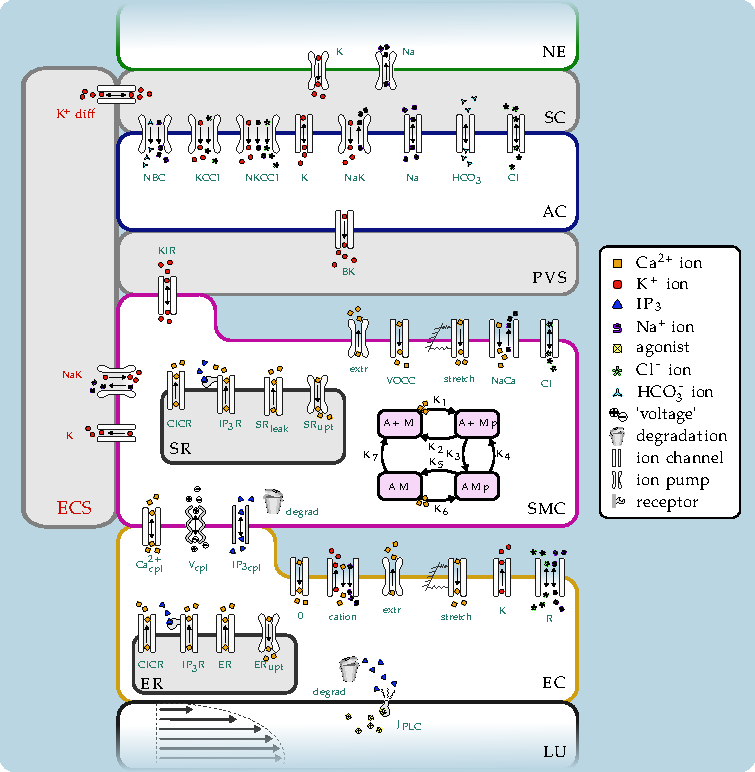
\includegraphics[width=1\linewidth]{new_figures/nvu_ecs}
		\caption{\textbf{NVU 1.1.1}. NE: neuron, SC: synaptic cleft, AC: astrocyte, PVS: perivascular space, SMC: smooth muscle cell, SR: sarcoplasmic reticulum, EC: endothelial cell, ER: endoplasmic reticulum, LU: lumen, ECS: extracellular space. $K_1$ to $K_7$: wall mechanics reaction rate constants, M: free nonphosphorylated cross bridges, Mp: free phosphorylated cross bridges, AMp: attached phosphorylated cross bridges, AM: attached dephosphorylated latch bridges, KIR: inwardly rectifying potassium channel, BK: large conductance potassium channel, VOCC: voltage operated calcium channel, CICR: calcium induced calcium release channel, IP$_3$R: $IP_3$ receptor calcium channel, $J_{PLC}$: phospholiphase-C dependent $IP_3$ flux, NaK: sodium potassium pump, K: calcium activated potassium channel. 
		The ECS compartment and fluxes $J_{\text{diff}}$, $J_{NaK}$ and $J_K$ shown in red are new additions to the NVU model.
		}
		\label{fig:nvu_ecs}
		\end{figure}
		
	It is proposed here that the interaction between the ECS and PVS compartment is excluded from the model, for the following reasons:
	it is assumed that the PVS volume is orders of magnitude smaller than the ECS as the astrocytic endfoot closely surrounds the arteriole \citep{Witthoft2012}. 
	In addition, by including a diffusive flux between the PVS and ECS in the model, the astrocytic $K^+$ pathway - where $K^+$ released into the SC during neuronal stimulation travels from the SC through the astrocyte and into the PVS - is effectively short circuited via the ECS and the astrocyte is bypassed.
	As such it is more physiologically realistic to model the PVS and ECS as completely separate spaces with no diffusive flux between them.
		
	 Diffusion of $K^+$ between the ECS and SC compartments of a single NVU is implemented via a linear diffusion term: 
		\begin{equation}
		J_{diff} = \frac{1}{\tau_s} \left( K_e - K_s \right),
		\label{eq:diffusion}
		\end{equation}
	
	where $J_{diff}$ is added to or subtracted from the differential equation for the $K^+$ concentration in the SC ($K_s$) and the $K^+$ concentration in the ECS ($K_e$) respectively. 
	$\tau_s$ is the characteristic time that is needed for $K^+$ to diffuse over some distance $\Delta x$:
		\begin{equation}
		\tau = \frac{(\Delta x)^2}{2D_K}, \; \; 		D_K = \frac{D_{free}}{\lambda_0^2}.
		\label{eq:tau}
		\end{equation}
		
	Here $D_K$ is the effective diffusion coefficient of $K^+$, $D_{free}$ is the diffusion coefficient of $K^+$ in a free medium, and $\lambda_0^2$ is a tortuosity factor which is necessary because diffusion is hindered by the narrow confines of the ECS \citep{Sykova2008}. 

	For diffusion between the ECS and SC, $\tau_s = 2.8$ based on an average astrocyte length (across two astrocyte arms) of $100 \; \mu m$. 
	The ECS is directly connected to the SMC via a calcium activated $K^+$ channel and sodium potassium pump (with fluxes denoted by $J_K$ and $J_{NaK}$ respectively) given by:
		\begin{align}
		J_K &= G_K w_i (v_i - v_K) \\
		J_{NaK} &= F_{NaK}.
		\end{align}
	
	\subsubsection{Extracellular Diffusion in the Tissue Slice (parBrain)}
		The macro scale simulations incorporate $K^+$ diffusion between the ECS of adjacent NVU tissue blocks via a linear diffusion term as in Equation \eqref{eq:diffusion} with characteristic time $\tau_e$. \cite{Dormanns2015b} estimated a tissue block size of diameter 400 $\mu$m, however arterioles of the cortex perfuse a cylindrical volume of diameter 140 to 320 $\mu$m \citep{boas}. Using the cylindrical diameter value of 140 $\mu$m and assuming that the cube shaped tissue blocks each containing a leaf of the H tree (arteriole) perfuse the same volume, the diameter of the tissue blocks is 124 $\mu$m. Therefore the characteristic time based on Equation \ref{eq:tau} for $K^+$ to travel through the ECS from one tissue block to another is $\tau_e = 4.3$ sec.  All relevant parameters are detailed in Table \ref{tab:csdpaper}.
		
				\begin{table}[h!]
					\small
					\centering
						\begin{tabular}{c c c l}
						\hline
						Parameter & Value & Unit & Description \\
						\hline
						$\tau_s$ & 2.8 & s & Characteristic time for diffusion between the SC and ECS \\
						$\tau_e$ & 4.3 & s & Characteristic time for diffusion between adjacent NVU tissue blocks \\
						$G_K$ & 4.46e-3 & $\mu M m V^{-1} s^{-1}$ & Whole SMC conductance for $K^+$ efflux \\
						$w_i$ & variable & - & Open state probability of calcium activated $K^+$ channel \\				
						$v_i$ & variable & mV & Membrane potential of the SMC \\
						$v_K$ & -94 & mV & Nernst potential \\		
						$F_{NaK}$ & 4.32e-2 & $\mu M s^{-1}$ & Rate of $K^+$ influx by the sodium potassium pump \\			
						\hline
						\end{tabular}
						\caption{Parameters of the NVU model with added ECS compartment.}
						\label{tab:csdpaper}
				\end{table}
		
		Diffusion between adjacent NVU tissue blocks is implemented using linear diffusion via the Laplace operator. Diffusion is not implemented for tissue blocks on a diagonal. For a single NVU with coordinates $i,j$ the equation for $K_e$ is given by
		
		\begin{equation}
		\frac{d K_e^{i,j}}{dt} = J_K^{i,j} - J_{NaK}^{i,j} - J_{diff}^{i,j} - \frac{1}{\tau_e} 
		\left( 4  K_e^{i,j} -  K_e^{i-1,j} - K_e^{i+1,j} - K_e^{i,j-1} - K_e^{i,j+1}
		\right).
		\end{equation}
		
		\subsubsection{Parallel Implementation}	
		Message Passing Interface (MPI) is used for the communication between tissue blocks in a multi-core architecture, where the MPI communication implements the extracellular diffusion. The simulated tissue slice is split into rectangular domains with each domain corresponding to a single core, whereas the H tree is partitioned into subtrees with a root subtree.
		For the extracellular diffusion, at each time step the state variables from the blocks along the edges of the domains are passed to the adjacent blocks in the neighbouring domain. Communication between domains and the corresponding boundary conditions enforcement within a single domain is implemented following the mesh ghost block communication pattern \citep{Gropp2014}. 